\documentclass[11pt,a4paper]{article}
\usepackage[margin=0.75in]{geometry}
\usepackage{titlesec}
\usepackage{enumitem}
\usepackage{xcolor}
\usepackage{hyperref}
\usepackage{graphicx}
\usepackage{fancyhdr}
\usepackage{tikz}
\usetikzlibrary{shapes,arrows,positioning}

\pagestyle{fancy}
\fancyhf{}
\rhead{NYU CDS Datathon 2025}
\lhead{HVAC Margin Rescue}
\cfoot{\thepage}

\titleformat{\section}{\normalfont\large\bfseries}{\thesection}{1em}{}
\titleformat{\subsection}{\normalfont\normalsize\bfseries}{\thesubsection}{1em}{}
\titlespacing*{\section}{0pt}{1.5ex}{1ex}
\titlespacing*{\subsection}{0pt}{1ex}{0.5ex}

\setlist[itemize]{noitemsep, topsep=2pt, leftmargin=*}
\setlist[enumerate]{noitemsep, topsep=2pt, leftmargin=*}

\begin{document}

\begin{center}
    {\LARGE \textbf{HVAC Margin Rescue: Technical Summary}} \\[0.3em]
    {\large Agentic Construction Financial Analytics Platform} \\[0.2em]
    {\small Autonomous analysis of \$6.4B portfolio (405 projects, 1.46M+ records)}
\end{center}

\vspace{-0.5em}
\hrule
\vspace{0.8em}

\section{System Architecture}

\begin{center}
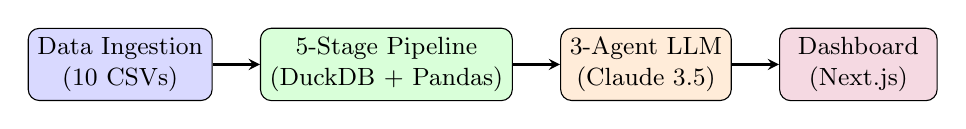
\begin{tikzpicture}[
    node distance=0.6cm,
    box/.style={rectangle, draw, rounded corners, minimum height=0.7cm, minimum width=2cm, font=\small, align=center},
    arrow/.style={->, >=stealth, thick}
]
    \node[box, fill=blue!15] (upload) {Data Ingestion\\(10 CSVs)};
    \node[box, fill=green!15, right=of upload] (pipeline) {5-Stage Pipeline\\(DuckDB + Pandas)};
    \node[box, fill=orange!15, right=of pipeline] (agents) {3-Agent LLM\\(Claude 3.5)};
    \node[box, fill=purple!15, right=of agents] (frontend) {Dashboard\\(Next.js)};

    \draw[arrow] (upload) -- (pipeline);
    \draw[arrow] (pipeline) -- (agents);
    \draw[arrow] (agents) -- (frontend);
\end{tikzpicture}
\end{center}

\textbf{Backend (FastAPI):} RESTful API with 5 routers---uploads, pipeline orchestration, portfolio queries, project analysis, and streaming chat. Async processing with background tasks and real-time progress callbacks.

\textbf{Frontend (Next.js + React):} Executive dashboard with 5 tabs (Summary, SOV, Labor/Material, Change Orders, Pipeline) plus drill-down project pages. Built with Shadcn/ui, Tailwind CSS, and Recharts.

\textbf{Data Pipeline:} Five-stage ETL---\textit{Clean} (role normalization), \textit{Load} (budget comparison), \textit{Enrich} (billing/CO/RFI), \textit{Flag \& Score} (risk identification), \textit{Export} (LLM packets).

\section{Agent Design}

Sequential 3-agent architecture with strict JSON output schemas:

\begin{enumerate}
    \item \textbf{Diagnosis Agent:} Forensic financial analysis identifying root causes (labor/material overruns, underbilling, rejected COs) with confidence scores (0.0--1.0). Outputs severity classification (CRITICAL/WARNING/WATCH) and recoverability assessment.

    \item \textbf{Recommendation Agent:} Generates ranked recovery actions with dollar quantification, urgency ratings, effort levels, and ROI estimates. Determines project mode (protect\_margin, accelerate\_cash, commercial\_recovery, closeout\_only).

    \item \textbf{Portfolio Optimization Agent:} Cross-project prioritization, resource allocation, GC negotiation bundling, and cash flow projections (7/30/60/90+ days). Produces globally-ranked action plan with weekly resource scheduling.
\end{enumerate}

\textbf{Packet Construction:} Hybrid context combining pre-computed metrics (1.2M labor logs $\rightarrow$ 6K summary rows), full field notes, change order details, and RFI data---optimized for token budget.

\section{AI Approach}

\textbf{Model:} Claude 3.5 Sonnet via Anthropic SDK with configurable token limits (4K analysis, 2K chat).

\textbf{Prompt Engineering:} System prompts defined in markdown files with strict JSON output schemas. Diagnostic signals and thresholds from centralized constants guide agent reasoning---ensuring fact-based analysis over generic commentary.

\textbf{Key Techniques:}
\begin{itemize}
    \item \textbf{Pre-aggregation:} Pipeline reduces raw data before LLM to prevent hallucination
    \item \textbf{Structured Output:} Regex-based JSON extraction with fallback parsing
    \item \textbf{Confidence Scoring:} Each root cause includes quantified confidence
    \item \textbf{Citation Requirement:} Agents must reference specific data points for all claims
    \item \textbf{Streaming:} Async message streaming for interactive chat interface
\end{itemize}

\section{Key Technical Decisions}

\begin{tabular}{@{}p{3cm}p{11cm}@{}}
\textbf{Storage} & CSV files + DuckDB for aggregations (no central DB)---enables rapid iteration and full dataset portability \\[0.3em]
\textbf{Configuration} & All business rules centralized in \texttt{constants.py}: severity thresholds, overrun limits (material $>$150\%, labor $>$50\%), flagging triggers, risk scoring weights \\[0.3em]
\textbf{Deployment} & Multi-stage Docker build (Node 20 + Python 3) on Railway.io; single container runs both FastAPI backend and Next.js standalone \\[0.3em]
\textbf{Caching} & In-memory CSV cache with \texttt{clear\_csv\_cache()} after uploads; atomic dataset swapping with backup/rollback \\[0.3em]
\textbf{Risk Scoring} & Percentile-based composite: Billing (40\%) + Margin (30\%) + Change Orders (20\%) + RFI (10\%) \\[0.3em]
\textbf{Error Handling} & Graceful degradation for optional files; 8 of 10 input CSVs are optional with fallback logic
\end{tabular}

\vspace{0.8em}
\hrule
\vspace{0.3em}
\begin{center}
\small\textit{Stack: FastAPI $\cdot$ Next.js $\cdot$ DuckDB $\cdot$ Pandas $\cdot$ Claude 3.5 Sonnet $\cdot$ Docker $\cdot$ Railway}
\end{center}

\end{document}
